% ----------------------------------------------------------
\chapter{Paleta de cores da FATEC}\label{anx:coresfatec}
% ----------------------------------------------------------

A paleta de cores da FATEC, disponível na \cpageref{marcafatec.1} a seguir, foi extraída do \emph{manual de identidade visual}\footnote{Disponível em \url{https://drive.google.com/file/d/0B1PtF63UJtuaZUFaU1VZTWt3YUk/view?resourcekey=0-o3NqvXakIULGhsMMyvn1Gg}} da FATEC Pompéia.

Note que, de acordo com a ABNT, a principal diferença entre anexo e apêndice é que os apêndices são textos criados pelo próprio autor para complementar sua argumentação, enquanto os anexos são documentos criados por terceiros, e usados pelo autor.

\cleardoublepage

\newcounter{includepdfpage} % para referenciar no texto páginas pdf incluídas

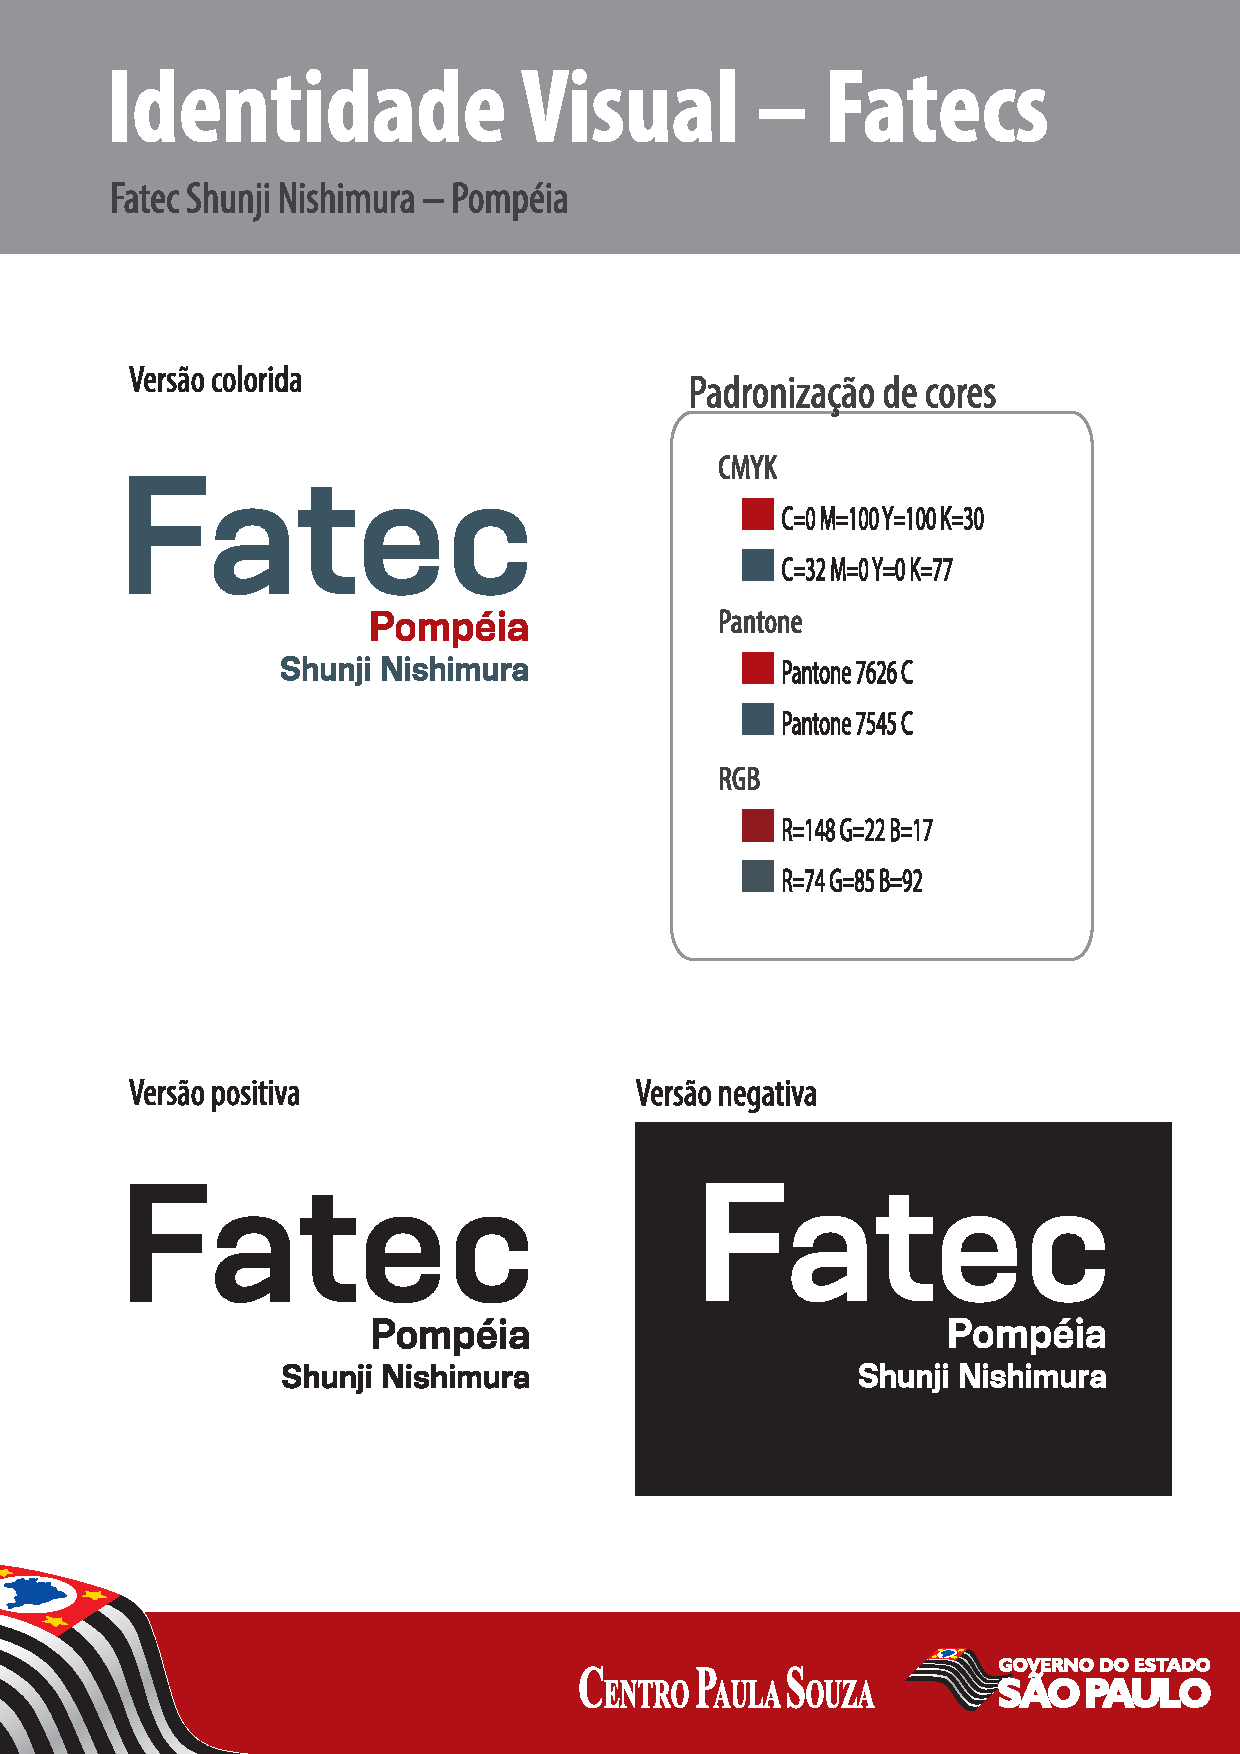
\includepdf[
    pages=-, % intervalo das páginas do arquivo pdf que serão incluídas
    scale=1, % controla o tamanho da página inserida
    pagecommand={\thispagestyle{plain} % imprime o número da página
    \refstepcounter{includepdfpage} % conta a página incluída
    \label{marcafatec.\theincludepdfpage} % marcaunb.n, n número da página
    },
    ]{fatectex-example/figuras/coresfatec}

\cleardoublepage